\section{Implementation}
\subsection{Simulated Network}

\subsubsection{Controller}

\subsubsection{Actuator}

\subsubsection{Sensor}

\subsubsection{Internet Cloud}

\subsubsection{Factory Access Point}

\subsubsection{Factory Bridge}

\subsection{MATLAB Simulation}
  Our MATLAB both simulated a system and a controler of the
  Tennessee Eastman problem, and used a custom packet interface
  between C++ and MATLAB as explained below.

\subsubsection{Tennessee Eastman}
  We buit a custom simplified Tennesee Eastman model in MATLAB.  
  This was based off of a preexisting FORTRAN model, but was
  reimplemented in MATLAB for ease of use and reduced complexity 
  \citation{Ricker}.  Our model contains variable vectors, an
  input vector, a state vector, and an output vector. Then by 
  using the equations provided in Ricker\citation{Ricker}, the
  simulation simply takes in the input vector from OMNeT++, and
  outputs the output vector, which includes the sensor data, to
  OMNeT++ via the MATLAB bridge.

  On the other side of the network, we also implemented a 
  controller in MATLAB for the Tennesee Eastman system.  This
  used steady state calculations to determine the optimal controls.
  The controller would input the output vector from the Tennessee
  Eastman system via the MATLAB bridge, and output a set of input
  vectors to be transmitted across the network into the MATLAB
  bridge.

\subsection{C++ to MATLAB Bridge}

\begin{figure*}
        \centering
		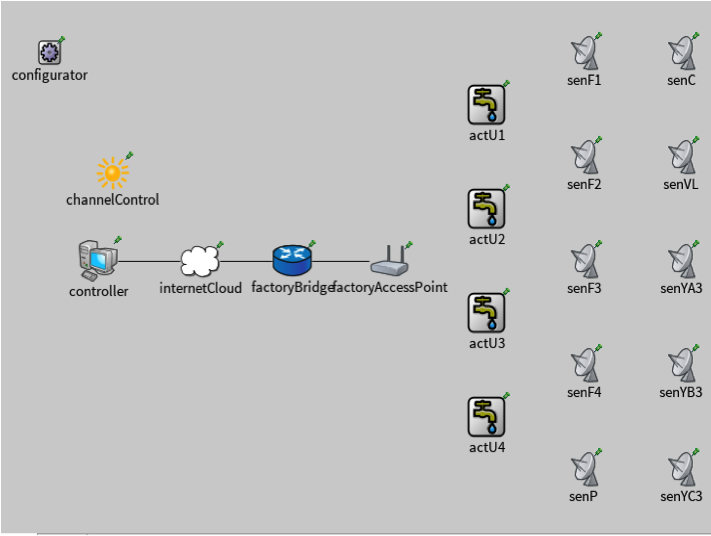
\includegraphics[width=0.8\textwidth]{figs/network.png}
        \caption{Network Diagram.}
        \label{fig:network}        
\end{figure*}
